\chapter{YOLO}
\ac{yolo} ist ein populäres Objekt Erkennungsmodell, dass dafür bekannt ist besonders schnell und akkurat Objekte in Bildern zu erkennen. Dies liegt an der kleinen Modellgröße und den hohen Berechnungsgeschwindigkeiten. Des Weiteren nutzt \ac{yolo} das gesamte Bild als Trainingsgrundlage, was es sowohl ermöglicht Videos zu klassifizieren als auch die Fehlerrate reduziert, dass der Hintergrund als Teil des Objektes klassifiziert wird. In diesem Kapitel geht es darum wie die Schnittstelle bzw. der Algorithmus gefüttert werden muss und was der Algorithmus für Datenformate erwartet \cite{Jiang.2022}.

\begin{wrapfigure}{r}{5cm}
    \includegraphics[width=4cm]{data/img/ordnerstruktur_yolo.png}
    \caption{Ordnerstruktur für einen Datensatz}
    \label{fig:folderYolo}
\end{wrapfigure}

Für die Studienarbeit wird der YOLOv5 von ultralytics \cite{glennjocher.2023} genommenm, da diese folgende Vorteile bietet:
\begin{itemize}
    \item aktive Developer am Projekt
    \item große Community 
    \item Docker deployable
    \item CUDA- und GPU-Unterstützung
    \item Pytorch Beschleungigung
\end{itemize}


\section{Generelle Ordnerstruktur}
Der \ac{yolo}-Algorithmus erwartet zum funktionieren eine generelle Ordnerstruktur, gezeigt in \ref{fig:folderYolo}. Der oberste Ordner ist dabei der Projektnameordner. In diesem müssen alle Projektrelevanten Bilder und Label enthalten sein. 

Auch darin enthalten sein muss das \textit{.yaml} file. Das wird in Kapitel \ref{sec:yaml_class} noch mal genauer beschrieben. Ansonsten müssen neben dem \textit{.yaml} file noch ein Ordner für die Trainingsdaten enthalten sein. Optional auch ein Testdatenordner und Validierungsdatenordner. Diese müssen wie der Trainingsdatenordner unter dem Projektordner eingeordnet werden.

Der Test, Train und Validordner müssen alle jeweils 2 Ordner haben für images und labels. Diese müssen auch über die verschiedenen Ordner exakt gleich benannt sein. Das heißt auch in der Groß- und Kleinschreibung. 

In dem images Ordner sind die vielen Testbilder enthalten, und in Labels die entsprechenden label dazu. Als Bildformate werden von dieser \ac{yolo} Version png, jpg und tiff Formate verarbeitet. Jeder Bildname muss einzigartig vorhanden sein (ich empfehle einfach die Bilder durchzunumerieren).

Bei den labeln werden nur .txt Dateien akzeptiert. Wichtig ist hier, dass die Daten zu einem Bild in einer gleichnamen .txt-Datei enthalten ist. Wenn als Beispiel ein Bild mit dem Namen \textit{test.jpg} vorhanden ist muss im Ordner labels auch das dazugehörige Labelfile \textit{test.txt} heißen.

\section{Aufbau der Label}
Jede Textdatei beinhaltet alle Label, die in dem dazugehörigen Bild zu finden sind. Dabei steht jede Zeile für ein Objekt das auf der Abbildung auffindbar ist. Diese können sich auch überlappen. Eine Zeile ist wie aufgebaut:
\begin{tcolorbox}
    \textless class\textgreater\space \textless x\_center\textgreater \space \textless y\_center\textgreater \space\textless width\textgreater \space\textless height\textgreater 
\end{tcolorbox}
\begin{figure}
    \begin{center}
        \includegraphics[width=8cm]{data/img/yolo_picture_structure.png}    
        \caption{Struktur YOLO Format veranschaulicht}
        \label{fig:yoloFormat}
    \end{center}
\end{figure}
Die "class" gibt an, welche Klasse das markierte Objekt hat. Die Klasse und dessen Name wird in dem YAML File definiert, worin auch angegeben wird wie viele Klassen es insgesamt gibt aber das wird in \ref{sec:yaml_class} noch einmal genauer erklärt. Der \textit{x\_center} gibt den Mittelpunkt des Labels an entlang der x-Achse (horizontal). \textit{y\_center} gibt das gleiche in der Vertikalen Richtung an. Genau kann das im Bild \ref{fig:yoloFormat} sehen. Der Punkt in der Mitte ist definiert durch \textit{x\_center} und \textit{y\_center}. Die komplette Breite und Lange wird entsprechend durch \textit{width} und \textit{height} dargestellt. 

Insgesamt werden alle Maße nicht in der px Anzahl dargestellt. Es wird dargestellt als das Verhältnis von der Länge/ Breite zur Gesamtlänge und -breite. Es wird dargestellt als eine \textit{float}-Nummer zwischen 0 und 1. Bei dem \textit{x\_center} und \textit{y\_center} wird zwischen den Punkt und dem Nullpunkt die Länge und Verhältnis zum gesamten Bild genommen in der entsprechenden Dimension. 

\section{YAML Klassifizierungsfile}
\label{sec:yaml_class}

Für jedes Projekt gibt es im Basis Folder ein \textit{.yaml} File mit einem selbstgewählten Namen. Dieses File besteht aus drei Teilen. Diese sind wie folgt aufgebaut:
\begin{verbatim}
    path: <path-to-yolo>
    train: <rel-path-to-train-dir>
    val: <rel-path-to-val-dir>

    names:
        0: <name>
        ...
\end{verbatim}

\textless rel-path-to-train-dir\textgreater ist der relative Pfad zum Trainingsdatensatz. Wenn der Standarttrainingssatzaufbau wie in Abbildung \ref{fig:folderYolo} aufgesetzt ist, dann ist dies \textit{./train/}. Der Pfad für den Validierungsdatensatz \textless rel-path-to-val-dir\textgreater ist ähnlich zu dem Trainingsdatensatzpfad. Beim Standardformat wäre es \textit{./valid/}. Der Pfad gibt den momentan Pfad an. Dieser wird durch die API ersetzt und kann standardisiert mit einem  \glqq .\grqq angegeben.

Unter \textit{names} werden die Namen aller relevanten Klassen angegeben. Dies sind die Klassen der jeweiligen Label und deren Bedeutung. Das heißt für ein Label einer Roten und gelben Ampel die geradeaus führt würde es Beispielsweise heißen \textit{0: rot-gelb-geradeaus}. Alle Label werden aufsteigend nummeriert. Die jeweilige Nummer in dem YAML File muss mit der jeweiligen Nummer in den \textit{.txt} Files übereinstimmen. Wenn die Nummer dieselbe ist, geht der YOLO-Aglorithmus aus, dass die jeweilige Nummer des Labels den Text beschreibt der im \textit{.yaml} File steht.